\documentclass[11pt,a4paper]{article}
\usepackage[utf8]{inputenc}
\usepackage[margin=25mm]{geometry}
\usepackage{amsmath}
\usepackage{array,booktabs,tabularx,longtable}
\usepackage{enumitem}
\usepackage{tikz}
\usetikzlibrary{arrows.meta,positioning}
\usepackage{listings}
\PassOptionsToPackage{hyphens}{url}
\usepackage[hidelinks]{hyperref}

% Keep the article's default Computer Modern serif family.
% All text, rules, diagrams, and links are black on white.
\urlstyle{rm}
\lstset{
  basicstyle=\small\rmfamily,
  columns=fullflexible,
  keepspaces=true,
  breaklines=true,
  showstringspaces=false,
  frame=single,
  framerule=0.3pt,
  xleftmargin=4pt,
  xrightmargin=4pt,
  aboveskip=8pt,
  belowskip=8pt
}
\setlength{\parindent}{0pt}
\setlength{\parskip}{6pt}
\setlength{\emergencystretch}{2em}
\renewcommand{\arraystretch}{1.2}
\setlist{itemsep=3pt,topsep=5pt}
\newcolumntype{Y}{>{\raggedright\arraybackslash}X}
\newcommand{\temp}[1]{\ensuremath{#1\,^{\circ}\mathrm{C}}}
\newcommand{\file}[1]{\nolinkurl{#1}}

\title{IoT-Based Smart Classroom\\
Energy Monitoring and Control System\\[5pt]
\large A Step-by-Step Guide to the Simulation Diagram}
\author{Project Documentation}
\date{19 November 2026}

\begin{document}
\maketitle

\begin{abstract}
This project uses an ESP32 to decide when classroom lighting, a fan, and a
cooling output should operate. Three sensors provide illumination,
motion, and temperature readings. The ESP32 applies local rules and
switches three relays. Animated appliance graphics make the relay outputs
visible in Wokwi. MQTT connects the controller to a backend and dashboard
for monitoring and manual commands. Energy is estimated from nominal
appliance power and recorded operating time; it is not measured by an
electrical energy meter.
\end{abstract}

\section{Start with the diagram}
\label{sec:orientation}
Open \file{diagram.json} at the repository root. An identical copy is
provided at \file{apps/firmware/diagram.json}. Keep the diagram visible
while reading this guide.

Read its numbered columns from left to right:
\begin{enumerate}
  \item \textbf{01 Sensors:} collect information about the room.
  \item \textbf{02 ESP32:} decide whether each output should be ON or OFF.
  \item \textbf{03 Relays:} switch the electrical signal sent to each visual.
  \item \textbf{04 Appliances:} show the resulting cooling, fan, and lighting states.
\end{enumerate}

The input and output rows are deliberately different. On the left,
\textbf{LDR is at the top, PIR is in the middle, and DHT22 is at the
bottom}. On the right, \textbf{cooling is at the top, fan is in the
middle, and lighting is at the bottom}. Horizontal position alone does
not mean that a sensor controls the appliance in the same row. For
example, the top-left LDR affects the bottom-right lighting output.
The ESP32 connects the meaning of the inputs to the appropriate outputs.

The short labels beside components identify their purpose and GPIO.
The labels beside appliances show nominal power and switching thresholds.
The footer gives shared rules and the power legend; the longer
explanations belong in this document.

\begin{figure}[htbp]
\centering
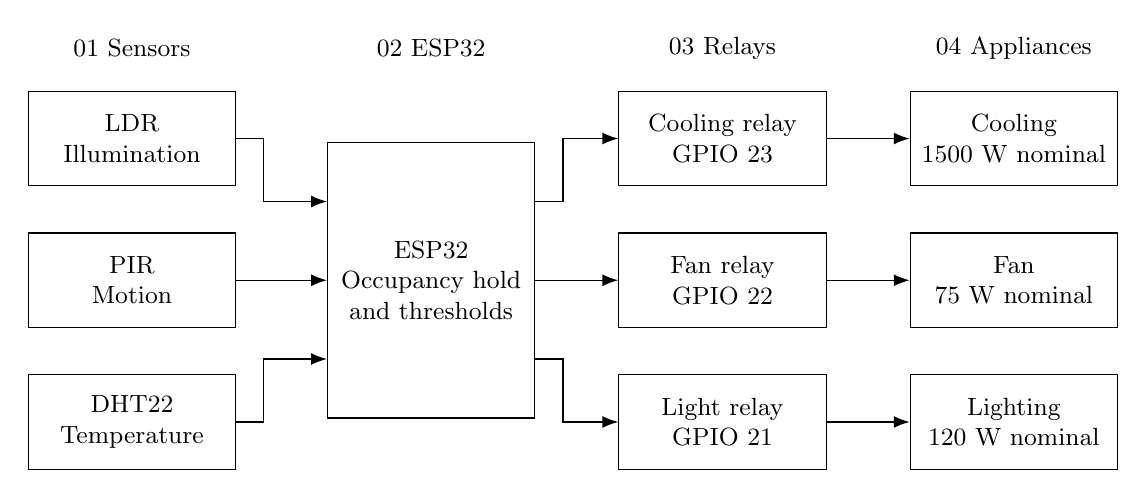
\begin{tikzpicture}[
  font=\small,
  block/.style={draw,rectangle,align=center,minimum height=12mm,text width=24mm},
  signal/.style={-{Latex[length=2mm]},line width=0.4pt}
]
\node at (0,1.15) {01 Sensors};
\node at (3.8,1.15) {02 ESP32};
\node at (7.5,1.15) {03 Relays};
\node at (11.2,1.15) {04 Appliances};
\node[block] (ldr) at (0,0) {LDR\\Illumination};
\node[block] (pir) at (0,-1.8) {PIR\\Motion};
\node[block] (dht) at (0,-3.6) {DHT22\\Temperature};
\node[block,minimum height=35mm] (esp) at (3.8,-1.8)
  {ESP32\\Occupancy hold\\and thresholds};
\node[block] (rc) at (7.5,0) {Cooling relay\\GPIO 23};
\node[block] (rf) at (7.5,-1.8) {Fan relay\\GPIO 22};
\node[block] (rl) at (7.5,-3.6) {Light relay\\GPIO 21};
\node[block] (ac) at (11.2,0) {Cooling\\1500 W nominal};
\node[block] (fan) at (11.2,-1.8) {Fan\\75 W nominal};
\node[block] (light) at (11.2,-3.6) {Lighting\\120 W nominal};
\draw[signal] (ldr.east) -- ++(0.35,0) |- ([yshift=10mm]esp.west);
\draw[signal] (pir.east) -- (esp.west);
\draw[signal] (dht.east) -- ++(0.35,0) |- ([yshift=-10mm]esp.west);
\draw[signal] ([yshift=10mm]esp.east) -- ++(0.35,0) |- (rc.west);
\draw[signal] (esp.east) -- (rf.west);
\draw[signal] ([yshift=-10mm]esp.east) -- ++(0.35,0) |- (rl.west);
\draw[signal] (rc.east) -- (ac.west);
\draw[signal] (rf.east) -- (fan.west);
\draw[signal] (rl.east) -- (light.west);
\end{tikzpicture}
\caption{A black-and-white reading map of the supplied diagram. This shows
the information path and actual row order; it is not a replacement for
the pin-by-pin circuit wiring. Power and ground connections are omitted
here for clarity.}
\label{fig:map}
\end{figure}

\section{What problem the project addresses}
A classroom can consume unnecessary energy when equipment stays on
during vacancies, when daylight is already sufficient, or when the room
does not need additional ventilation or cooling. The project tests
whether combining occupancy, illumination, and temperature information
can reduce unnecessary operating time.

The controller makes three separate decisions: whether lighting is
needed, whether the fan is needed, and whether cooling is needed. In the
default SMART mode, all three decisions first require effective
occupancy. The project also provides a CONVENTIONAL baseline and a MANUAL
mode so the behavior can be demonstrated and compared.

The simulation demonstrates the control logic. The offline experiments
replay room scenarios for repeatable comparisons. Neither approach
establishes measured savings in a real classroom without a separate
physical study.

\section{Column 01: understand the three sensors}
\subsection{Top-left: LDR illumination sensor}
The LDR module represents the amount of light already present in the
room. Its \textbf{AO} pin is the analog output connected to
\textbf{GPIO 34}. An analog value can vary over a range; it is not limited
to a simple ON/OFF signal. The ESP32 reads this value with its
analog-to-digital converter and converts it to approximate lux.

\textbf{Lux} is the illumination value used by the lighting rule. A low
value represents a darker room. In this diagram the initial setting is
\textbf{100 lux}, which is below the lighting ON threshold. Nevertheless,
the light remains OFF until occupancy is detected in SMART mode.

The module is supplied from 3.3 V. Its digital output, DO, is unused.
The firmware uses AO because it needs illumination values for two
different thresholds. To change the room brightness, click the LDR in
Wokwi and adjust its illumination setting. The conversion is an
approximation and is not a calibrated classroom light measurement.

\subsection{Middle-left: PIR motion sensor}
The PIR provides a digital signal on \textbf{OUT}, connected to
\textbf{GPIO 13}. HIGH means the sensor is reporting motion; LOW means it
is not currently reporting motion. To create an event, click the PIR
and select \textbf{Simulate Motion}.

Motion is not the same as a reliable count of people. A seated person
may remain still. The firmware therefore remembers recent motion using
an \textbf{occupancy hold}: the room remains effectively occupied for
15 seconds after the last HIGH signal in the simulation.

The diagram's PIR HIGH pulse lasts 2 seconds. Consequently, an isolated
button click can keep outputs active for approximately 17 seconds:
about 2 seconds of HIGH followed by a 15-second hold. The hold is
refreshed while HIGH continues, so do not measure the 15 seconds from
the initial mouse click. Repeat motion to keep the room occupied during
a longer demonstration.

\subsection{Bottom-left: DHT22 temperature and humidity sensor}
The DHT22 data pin is named \textbf{SDA} in the diagram and connects to
\textbf{GPIO 15}. Here SDA is the DHT22 data connection; it does not mean
that this sensor uses an I\textsuperscript{2}C bus.

Temperature determines the fan and cooling decisions. Humidity is also
read and transmitted, but it does not switch any appliance in the
current policy. The initial values are \textbf{\temp{29}} and
\textbf{60\% humidity}. Click the DHT22 to change these inputs.

Turning cooling ON does not make the simulated DHT22 temperature fall.
The input must be changed manually, or supplied by an experiment
scenario. This distinction matters when explaining what the simulation
has demonstrated.

\section{Column 02: understand the ESP32}
\subsection{GPIO names and the complete signal map}
A GPIO is a general-purpose input/output connection on the controller.
The number in a label is the GPIO number, not the physical position of
the pin on the board. Use the printed pin names when following a wire.

\begin{table}[htbp]
\centering
\begin{tabularx}{\textwidth}{@{}l l Y@{}}
\toprule
Signal connection & ESP32 GPIO & What passes through it \\
\midrule
LDR AO & 34 & Analog illumination input \\
PIR OUT & 13 & Digital motion input \\
DHT22 SDA & 15 & Temperature and humidity data \\
Light relay IN & 21 & Lighting ON/OFF command \\
Fan relay IN & 22 & Fan ON/OFF command \\
Cooling relay IN & 23 & Cooling ON/OFF command \\
\bottomrule
\end{tabularx}
\caption{Signal connections used by the supplied firmware and diagram.}
\label{tab:pins}
\end{table}

\subsection{What happens in one controller cycle}
The ESP32 starts in SMART mode with its output commands OFF. In its
main loop it reads the PIR signal and updates effective occupancy.
It refreshes temperature, humidity, and illumination readings about
every 2 seconds, evaluates the rules, and changes the outputs when
necessary. It also records operating time and attempts network work.

Telemetry is scheduled every 3 seconds when MQTT is available, and
serial status is printed every 5 seconds. These are different activities:
a relay can change before the next status line appears. The timing is
intended for this demonstration, not a hard real-time guarantee.

Automatic decisions are made on the ESP32. The backend does not calculate
the SMART relay commands. The local demonstration can run with MQTT
offline, although network connection attempts may introduce delays.

\subsection{The occupancy condition}
In SMART mode, effective occupancy is checked before the illumination
and temperature rules. If the room is unoccupied, all three outputs are
OFF even if it is hot and dark. If motion is detected, the controller
evaluates which outputs are needed. When the hold expires, all three
outputs turn OFF.

The 15-second hold is selected by the firmware's simulation setting.
The physical-mode setting and offline experiments use
\textbf{600 seconds (10 minutes)}. Changing a backend setting does not
automatically change the compiled ESP32 policy.

\section{Columns 03 and 04: trace a relay to an appliance}
\subsection{Control side and contact side}
Each relay has two jobs that must be read separately. On the control
side, \textbf{IN} receives the GPIO command, while \textbf{VCC} and
\textbf{GND} supply the relay module. On the contact side, \textbf{COM}
is the common terminal, \textbf{NO} is the normally open terminal, and
\textbf{NC} is the normally closed terminal.

In this circuit, COM is supplied with 3.3 V and NO connects to the
appliance visual's SW input. NC is unused. When COM and NO are connected,
SW receives a HIGH signal and the visual shows ON. When the contact
opens, the visual's internal pull-down makes SW LOW and the visual
shows OFF. This avoids a floating input retaining an ambiguous state.

The firmware uses active-HIGH commands and the supplied Wokwi relay
model uses the \emph{pnp} attribute. These settings describe this
particular simulated configuration; do not infer the wiring or trigger
polarity of a different physical relay board from the attribute name.

\subsection{Follow one complete example: the fan}
\begin{enumerate}
  \item Locate the middle-left PIR. Its OUT signal tells GPIO 13 about motion.
  \item Locate the bottom-left DHT22. Its SDA signal gives GPIO 15 the
  temperature reading.
  \item The ESP32 checks effective occupancy and the fan thresholds.
  If the fan was OFF, an occupied room at \temp{28} or above requests ON.
  \item GPIO 22 drives IN on the middle relay.
  \item The relay's COM--NO path supplies the fan visual's SW input.
  \item The middle-right display shows ON and its blades animate.
\end{enumerate}
The same path applies to lighting and cooling, using GPIO 21 and GPIO
23 respectively. Lighting uses lux; cooling uses temperature.

\subsection{What the appliance drawings actually mean}
The right-hand components are custom Wokwi visuals. Lighting uses a
fixture with illuminated tubes, the fan uses moving blades, and cooling
uses a wall-unit drawing with moving airflow. Each visual also has an
ON/OFF badge. They observe the relay contacts; they are not additional
hardware displays driven by new ESP32 output pins.

The labels 120 W, 75 W, and 1500 W are \textbf{nominal power assumptions}
used in energy calculations. The visual's 3.3 V input is only a state
signal. It does not represent the actual electrical supply or current
of a classroom lamp, motor, or air conditioner. The current diagram has
three controlled outputs; it has no implemented projector channel.

\section{Read the power and wiring correctly}
\begin{table}[htbp]
\centering
\begin{tabularx}{\textwidth}{@{}l Y@{}}
\toprule
Supply or return & Where it is used \\
\midrule
3.3 V & DHT22 VCC, LDR VCC, and all three relay COM terminals \\
5 V & PIR VCC and the VCC terminals of the three relay modules \\
Ground & Sensor returns, relay GND, and appliance visual GND \\
\bottomrule
\end{tabularx}
\caption{Power distribution in the simulation.}
\end{table}

The on-screen wire legend uses red for 3.3 V, purple for 5 V, and black
for ground. Cyan identifies sensor signals. Orange, green, and blue
identify lighting, fan, and cooling paths. This document remains
black and white: use the endpoint names in Table~\ref{tab:pins}, rather
than relying on colour.

The long vertical wires distribute a shared supply or return between
components. They do not mean that all outputs receive the same control
command. IN and NO connections remain separate for each appliance.
Likewise, a drawn crossing does not by itself create an electrical
connection in the JSON diagram. The specified pin endpoints determine
the connections.

The supplied circuit is a low-voltage simulation representation. It is
not a mains-installation drawing or a specification for driving real
classroom appliances directly from an ESP32.

\section{The exact SMART rules}
\label{sec:rules}
\begin{table}[htbp]
\centering
\begin{tabularx}{\textwidth}{@{}l Y Y@{}}
\toprule
Output & Turn ON when currently OFF & Turn OFF when currently ON \\
\midrule
Lighting & Occupied and lux \(\leq 150\) & Lux \(\geq 250\), or vacancy timeout \\
Fan & Occupied and temperature \(\geq\temp{28}\) & Temperature \(\leq\temp{26}\), or vacancy timeout \\
Cooling & Occupied and temperature \(\geq\temp{29}\) & Temperature \(\leq\temp{28}\), or vacancy timeout \\
\bottomrule
\end{tabularx}
\caption{The thresholds are inclusive at the stated ON and OFF limits.
These rules apply to SMART mode.}
\end{table}

\subsection{Why ON and OFF use different thresholds}
The gap between the thresholds is called \textbf{hysteresis}. Within
that gap, the device keeps its previous state. This reduces repeated
switching when a reading fluctuates near a boundary.

For lighting, the gap is between 150 and 250 lux. At 200 lux, an already
ON light stays ON, while an already OFF light stays OFF. At exactly
150 lux, an OFF light turns ON; at exactly 250 lux, an ON light turns
OFF. The previous state therefore matters when predicting a result.

For the fan, \temp{27} lies inside the hold band. For cooling,
\temp{28.5} lies inside its hold band. Fan and cooling decisions are
independent: both can be ON together. Cooling is not implemented as a
replacement that automatically turns the fan OFF.

\subsection{A complete room example}
At startup, the diagram is set to \temp{29} and 100 lux, but no motion
has been detected. All outputs are OFF. Trigger motion: the room becomes
effectively occupied, 100 lux requests lighting, \temp{29} requests the
fan, and \temp{29} also requests cooling. All three outputs become ON.

Now set the temperature to \temp{28}. Cooling turns OFF at its OFF
threshold, but the fan remains ON because it is still above \temp{26}.
Set illumination to 300 lux and lighting turns OFF. Finally, stop
motion and allow the occupancy hold to expire; the fan also turns OFF.

\section{Operating modes}
\begin{description}[style=nextline]
  \item[SMART --- the default]
  Uses occupancy, lux, temperature, and hysteresis as described above.
  This is the mode to use when demonstrating automatic decisions.
  \item[CONVENTIONAL --- the comparison baseline]
  Keeps all three outputs ON regardless of occupancy, temperature, or
  daylight. It represents the project's defined scheduled-operation
  baseline, not every real classroom's operating practice.
  \item[MANUAL --- direct demonstration control]
  Keeps the selected output states and accepts explicit ON/OFF commands
  from the dashboard through MQTT. Selecting MANUAL does not itself
  reset every output to OFF. The firmware rejects direct device commands
  unless MANUAL is selected.
\end{description}

The automatic thresholds printed beside appliances are SMART-mode
rules. They do not override CONVENTIONAL or MANUAL mode.

\section{Run the local Wokwi demonstration}
\label{sec:run}
\subsection{Prepare and start}
Use VS Code with the Wokwi extension and a valid Wokwi license, plus
PlatformIO for the ESP32 build. Open the repository root as the
workspace, then run:
\begin{lstlisting}
pio run -d apps/firmware
\end{lstlisting}
Press F1 and select \textbf{Wokwi: Start Simulator}. If the simulator
opens at its idle screen, press its green play button. Opening
\file{apps/firmware} as the workspace also works; its configuration
points to the same build and custom visual binary.

The custom appliance WASM binary is included in the repository. It does
not need to be rebuilt just to run the demonstration. The ESP32
firmware is built locally; its generated \file{.pio} directory is not
part of the source distribution.

\subsection{Check the initial state}
After startup, allow a few seconds for a valid sensor reading.
At the initial \temp{29} and 100 lux, the room should still be
unoccupied and all outputs should be OFF. This is the first check that
the occupancy condition is working.

Open the Wokwi terminal and look for a status line containing:
\begin{lstlisting}
mode=SMART occupancy=UNOCCUPIED temp=29.0C lux=100
light=OFF fan=OFF cooling=OFF
\end{lstlisting}
The actual line also includes estimated energy and MQTT connection
status. Line wrapping depends on the terminal width.

\subsection{Run the following cases}
Before each occupied case, click PIR and select \textbf{Simulate Motion}.
Repeat motion if the case takes longer than the hold period. After
changing temperature or lux, allow at least one sensor sampling interval
of about 2 seconds. Also allow time for the next serial status line.

\begin{longtable}{@{}p{0.08\textwidth}p{0.43\textwidth}p{0.41\textwidth}@{}}
\toprule
Case & What to do & Expected SMART result \\
\midrule
\endfirsthead
\toprule
Case & What to do & Expected SMART result \\
\midrule
\endhead
1 & Leave the room unoccupied, even at \temp{29} and 100 lux. &
All three outputs OFF. \\
2 & Trigger motion at \temp{29} and 100 lux. &
Lighting, fan, and cooling ON. \\
3 & While occupied, set \temp{24} and 100 lux. &
Lighting ON; fan and cooling OFF. \\
4 & While occupied, set \temp{28} and 500 lux. &
Fan ON; lighting and cooling OFF. \\
5 & While occupied, set \temp{30} and 500 lux. &
Fan and cooling ON; lighting OFF. \\
6 & While occupied, change lux from 140 to 200 to 260, waiting after each change. &
Lighting ON, remains ON, then OFF. \\
7 & While occupied, change temperature from \temp{29} to \temp{28.5}
to \temp{28} to \temp{26}. &
Both thermal outputs ON; both stay ON; cooling OFF; then fan OFF. \\
8 & With outputs ON, stop triggering motion. &
All outputs OFF 15 seconds after the last PIR HIGH. \\
\bottomrule
\end{longtable}

The firmware reports state transitions with messages such as:
\begin{lstlisting}
[CONTROL] fan=ON reason=SMART_POLICY
[CONTROL] fan=OFF reason=OCCUPANCY_TIMEOUT
\end{lstlisting}
Check both the serial state and the corresponding appliance graphic.
A successful firmware message alone does not prove that a custom
visual or relay connection is correct.

\section{What the IoT connection adds}
\subsection{The path shown in the diagram footer}
The network path is:
\[
 \text{ESP32}\ \longleftrightarrow\ \text{MQTT broker}\
 \longleftrightarrow\ \text{backend}\
 \longleftrightarrow\ \text{dashboard}.
\]
The broker is Mosquitto. The backend is a FastAPI service that stores
observations in SQLite. The dashboard displays readings, states,
runtime, and estimated energy, and lets the user send mode and manual
commands. The browser polls the backend; it does not directly drive
the relay GPIOs.

\begin{table}[htbp]
\centering
\begin{tabularx}{\textwidth}{@{}l Y@{}}
\toprule
MQTT topic & Purpose and direction \\
\midrule
\nolinkurl{smartclassroom/telemetry} & ESP32 to backend: sensor readings, mode,
output states, runtimes, and estimated energy. \\
\nolinkurl{smartclassroom/mode} & Backend to ESP32: select SMART,
CONVENTIONAL, or MANUAL. \\
\nolinkurl{smartclassroom/control} & Backend to ESP32: request a device
state; applied only in MANUAL mode. \\
\bottomrule
\end{tabularx}
\end{table}

For example, a mode message is \lstinline|{"mode":"MANUAL"}|.
A device message is \lstinline|{"device":"fan","state":true}|.
The next telemetry sample confirms the applied state. Broker acceptance
of a message is not the same as confirmation that a relay has changed.

\subsection{Start the backend and dashboard}
For the full local system, use Python 3.11--3.13, uv, and
Mosquitto. Run commands from the repository root. Install dependencies:
\begin{lstlisting}
uv sync --project apps/server --extra dev --extra research
\end{lstlisting}
Start the broker in one terminal:
\begin{lstlisting}
mosquitto -c infra/mosquitto/mosquitto.conf -v
\end{lstlisting}
Start the backend in another terminal:
\begin{lstlisting}
uv run --project apps/server uvicorn smart_classroom_api.main:app --reload --host 127.0.0.1 --port 8000
\end{lstlisting}
Start Wokwi, then open \url{http://127.0.0.1:8000}.
The firmware uses \nolinkurl{host.wokwi.internal} on port 1883 to reach the
host's broker, which requires Wokwi's Private IoT Gateway. An
\lstinline|mqtt=OFFLINE| status means remote telemetry and commands are
unavailable; it does not itself mean that local SMART control has failed.

\section{Understand the energy estimate}
\label{sec:energy}
For each appliance, estimated energy is
\[
 E_i\,[\mathrm{Wh}] =
 P_i\,[\mathrm{W}]\,t_i\,[\mathrm{h}].
\]
The firmware records ON time and uses nominal ratings of 120 W for
lighting, 75 W for the fan, and 1500 W for cooling. Total estimated
energy is the sum of the three values.

For example, if all three run for exactly 10 minutes:
\begin{align*}
E_{\mathrm{light}} &= 120 \times \frac{10}{60} = 20\ \mathrm{Wh},\\
E_{\mathrm{fan}} &= 75 \times \frac{10}{60} = 12.5\ \mathrm{Wh},\\
E_{\mathrm{cooling}} &= 1500 \times \frac{10}{60} = 250\ \mathrm{Wh},\\
E_{\mathrm{total}} &= 282.5\ \mathrm{Wh} = 0.2825\ \mathrm{kWh}.
\end{align*}
This is a worked calculation, not a measured outcome of a particular
live run. W denotes power; Wh denotes accumulated energy. An appliance
being OFF stops adding runtime, but does not erase energy accumulated
earlier in the session.

The backend estimates interval energy from changes in cumulative
runtime counters and its configured ratings. Keep those ratings aligned
with the firmware when comparing live values. Firmware runtime counters
restart when the controller restarts; stored backend history is separate.

The offline experiments compare the same input scenarios under SMART
and CONVENTIONAL policies. When the conventional estimate is positive,
\[
 \text{Estimated saving (\%)} =
 \frac{E_{\mathrm{conventional}}-E_{\mathrm{smart}}}
 {E_{\mathrm{conventional}}}\times100.
\]
Lower estimated consumption in a scenario demonstrates reduced modeled
runtime. It does not, by itself, establish actual building electricity
savings or prove that real thermal comfort was achieved.

\section{Troubleshooting while looking at the diagram}
\begin{longtable}{@{}p{0.30\textwidth}p{0.62\textwidth}@{}}
\toprule
What you see & What to check first \\
\midrule
\endfirsthead
\toprule
What you see & What to check first \\
\midrule
\endhead
Everything is OFF in a hot, dark room. &
In SMART mode, trigger PIR motion. Temperature and darkness alone are
not enough without effective occupancy. \\
Outputs turn OFF while you adjust a sensor. &
The 15-second hold may have expired. Trigger motion again and wait for
the next sensor reading. \\
A device stays ON after a small input change. &
Check its OFF threshold. A value inside the hysteresis band preserves
the existing state. \\
Cooling stays ON at \temp{28.5}. &
This is expected if it was already ON; its OFF threshold is \temp{28}. \\
The fan stays ON when cooling starts. &
The two outputs are controlled independently. Both ON is a valid state. \\
All outputs remain ON despite vacancy. &
Check the operating mode. CONVENTIONAL deliberately ignores vacancy;
MANUAL follows selected states. \\
Cooling ON does not reduce temperature. &
The simulation has no room thermal-feedback model. Adjust the DHT22
input yourself. \\
Serial state changes but a visual does not. &
Trace the matching GPIO to relay IN and relay NO to the visual's SW.
Check COM supply, ground, and the custom-chip binary. \\
The simulator cannot find firmware. &
Build from the root using \lstinline|pio run -d apps/firmware|, and
use the supplied Wokwi configuration for the workspace you opened. \\
A custom-chip memory error appears. &
Use the bundled corrected WASM, or rebuild with the supplied script.
It explicitly limits stack allocation for Wokwi. \\
MQTT is OFFLINE or the dashboard has no readings. &
Check Mosquitto, the backend, port 1883, and Private IoT Gateway access.
First confirm local operation in the Wokwi terminal. \\
\bottomrule
\end{longtable}

\section{Implementation files and validation}
\subsection{Where each responsibility lives}
\begin{longtable}{@{}p{0.36\textwidth}p{0.56\textwidth}@{}}
\toprule
File or directory & Responsibility \\
\midrule
\endfirsthead
\toprule
File or directory & Responsibility \\
\midrule
\endhead
\file{diagram.json} &
Root-workspace circuit, component positions, wiring, and concise labels. \\
\file{apps/firmware/diagram.json} &
Authoritative matching circuit for the firmware workspace. \\
\file{apps/firmware/include/smart_classroom/config.h} &
GPIO mapping, timing, thresholds, nominal ratings, and MQTT topics. \\
\file{apps/firmware/src/sensors/} &
Sensor readings, approximate lux conversion, and occupancy hold. \\
\file{apps/firmware/src/control/} &
SMART rules, output transitions, runtime, and energy calculations. \\
\file{apps/firmware/src/connectivity/} &
Wi-Fi/MQTT connection handling and telemetry messages. \\
\file{apps/firmware/chips/} &
Custom appliance graphics, chip definition, API header, and bundled WASM. \\
\file{apps/server/} and \file{apps/dashboard/} &
Backend, stored observations, API, and browser monitoring/control. \\
\file{experiments/} &
Scenario replay, conventional comparison, and generated analysis. \\
\file{tools/build_appliance.py} &
Reproducible compilation of the custom visual component. \\
\file{tools/check_diagram.py} &
Diagram consistency and compiled-visual behavior checks. \\
\bottomrule
\end{longtable}

\subsection{Rebuild and check the custom visuals}
Only use the first command below when the graphics implementation has
changed. The second command checks the diagram copies, connections,
configured paths, and compiled display behavior:
\begin{lstlisting}
uv run --with ziglang==0.17.1 python tools/build_appliance.py
uv run --with wasmtime==44.0.0 python tools/check_diagram.py
\end{lstlisting}
The component reserves separate state for the circuit's three appliance
instances. It uses a 64 KiB stack and requires 9 WebAssembly memory
pages, below Wokwi's 64-page limit. Checks exercise ON/OFF transitions,
animation stopping at OFF, and display isolation when three instances
share a module. Adding more appliance instances would also require
updating this implementation and the rest of the device model.

\subsection{What has been verified}
The local VS Code simulation was started on 19 November 2026.
Serial output showed the initial unoccupied/OFF state, motion causing
all three commands to turn ON at \temp{29} and 100 lux, and the
occupancy timeout turning them OFF. The live run exposed memory-size
and shared-state issues in the custom visuals; both were corrected.
After correction, all three graphics loaded and displayed their active
states together.

The ESP32 build and the automated diagram/visual checks passed.
MQTT was offline during the local demonstration. Therefore the latest
local run does not verify the complete backend/dashboard path, every
manual test case, or physical appliance operation. The detailed record
is in \file{docs/validation.md}.

\subsection{Limits to keep in mind}
PIR detects motion rather than counting people. LDR lux is approximate.
There is no electrical power meter and no simulated room heat-flow
feedback. If DHT22 readings fail after earlier valid readings, the
sensor manager retains the last valid temperature and reports a sensor
error; the demonstration should not be presented as a validated
fail-safe physical controller.

These limits do not prevent the diagram from explaining the intended
control sequence: \textbf{sense the room, decide locally, switch a relay,
and observe the corresponding appliance state}.

\section*{Project and supporting documents}
\begin{itemize}
  \item Repository:
  \url{https://github.com/nazzmullxd/IoT-Based-Smart-Classroom-Energy-Monitoring-and-Control-System}
  \item Short diagram guide: \file{docs/diagram-guide.md}.
  \item Architecture and MQTT contract:
  \file{docs/architecture/architecture.md} and
  \file{docs/architecture/mqtt.md}.
  \item Test matrix and validation:
  \file{docs/test-plan.md} and \file{docs/validation.md}.
  \item Experiment methodology:
  \file{docs/thesis/methodology.md}.
\end{itemize}

\end{document}
